\documentclass[aspectratio=1610]{beamer}
%Information to be included in the title page:

\usetheme{Madrid}
\usepackage{amsmath}
\usepackage{amssymb}
\usepackage{listings}
\usepackage{xcolor}
\lstset{
  language=Python,  %代码语言使用的是matlab
  frame=shadowbox, %把代码用带有阴影的框圈起来
  rulesepcolor=\color{red!20!green!20!blue!20},%代码块边框为淡青色
  keywordstyle=\color{blue!90}\bfseries, %代码关键字的颜色为蓝色,粗体
  commentstyle=\color{red!10!green!70}\textit,    % 设置代码注释的颜色
  showstringspaces=true,%不显示代码字符串中间的空格标记
  numbers=left, % 显示行号
  numberstyle=\tiny,    % 行号字体
  numberstyle=\color{green},
  stringstyle=\rmfamily\slshape\color[RGB]{128,0,0}, % 代码字符串的特殊格式
  breaklines=true, %对过长的代码自动换行
  extendedchars=false,  %解决代码跨页时,章节标题,页眉等汉字不显示的问题
  escapeinside=``,%代码中出现中文必须加上,否则报错
  texcl=true}

\lstset{breaklines}%自动将长的代码行换行排版

\lstset{extendedchars=false}%解决代码跨页时,章节标题,页眉等汉字不显示的问题

\usepackage{textcomp}
% \usepackage[margin=1in]{geometry}
\usepackage{pythonhighlight}
% \usepackage{minted}
\usepackage[backend=bibtex]{biblatex}
%\usepackage[style=authortitle,backend=biber]{biblatex}
\addbibresource{references.bib}

\title{Sample title}
\author{Anonymous}
\institute{Overleaf}
\date{2021}

\begin{document}

\begin{frame}[plain]
  \titlepage
  %  Title page
\end{frame}
\section{induction}
\begin{frame}
  SIS, 
\end{frame}

\section{example}
\begin{frame}{problem}
  \begin{figure}[htbq]
    \centering
    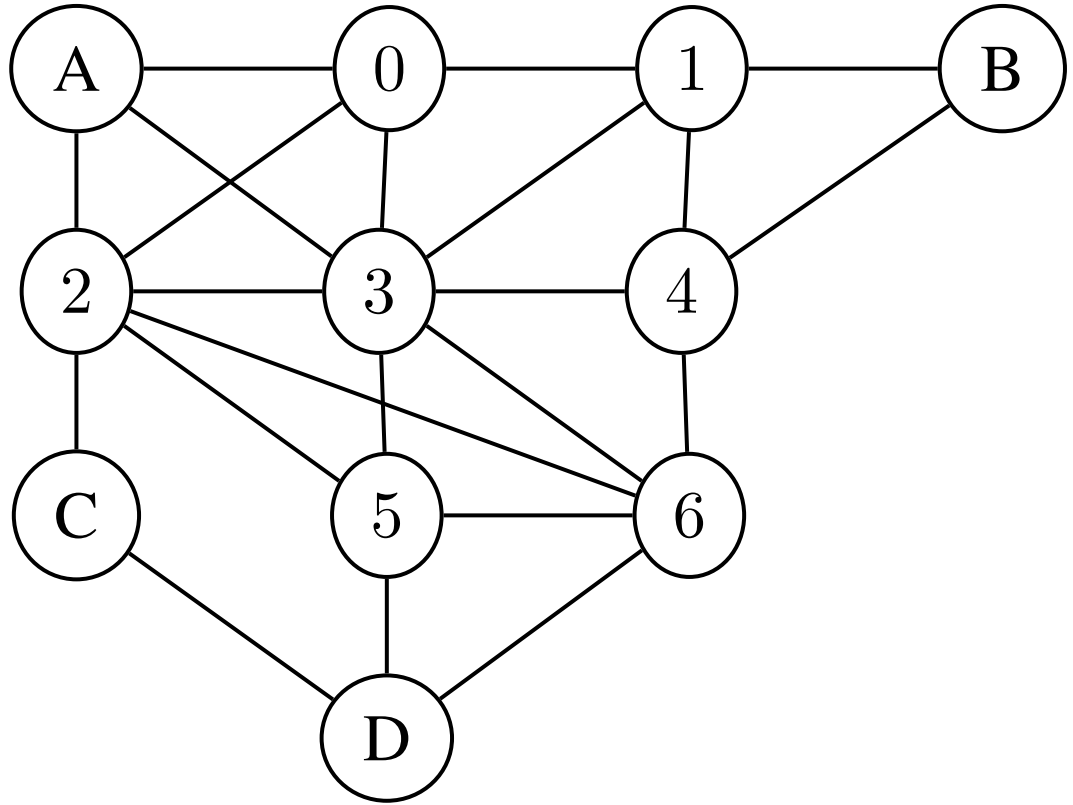
\includegraphics[width=0.5\textwidth]{problem.png}
    \caption{Zed city as an undirected graph} 
    \label{fig-zed}
  \end{figure}
\end{frame}
\begin{frame}{boolean function}
  \begin{columns}
    \begin{column}{0.5\linewidth}
      \begin{block}{python implementation of f }
        
      \end{block}
    \end{column}
    \begin{column}{0.5\linewidth}
      \begin{figure}[htbq]
        \centering
        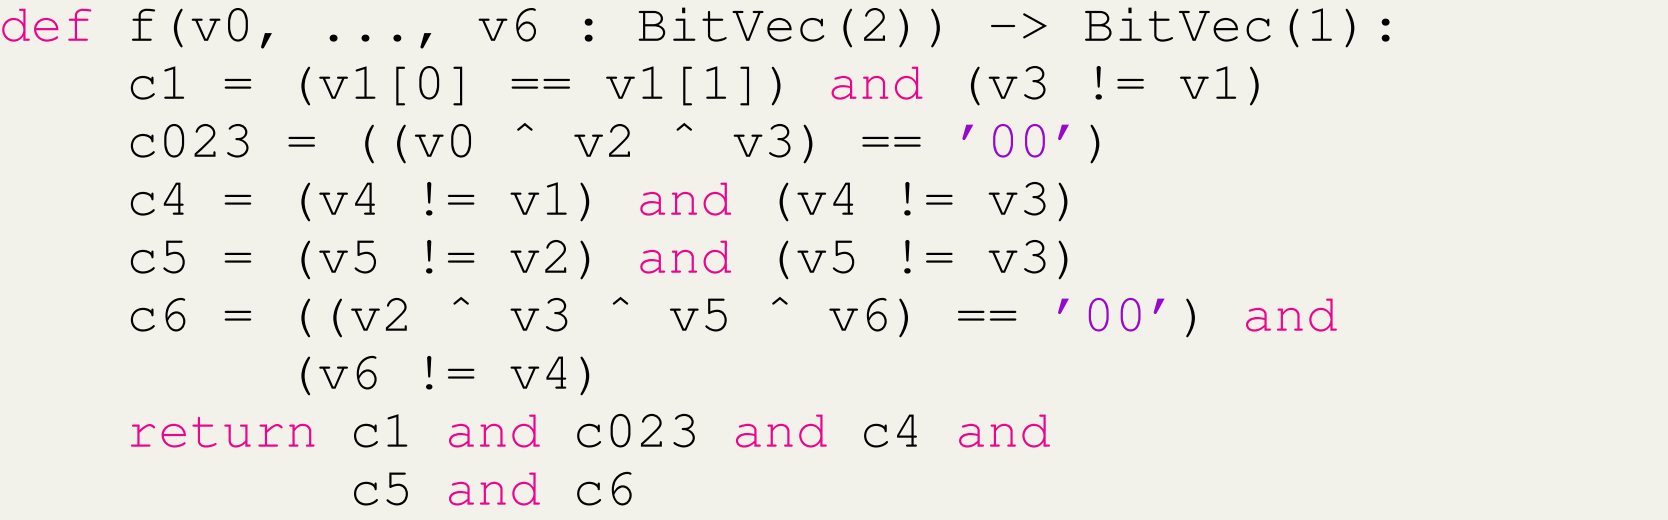
\includegraphics[width=\textwidth]{code2.png}
      \end{figure}
    \end{column}
  \end{columns}
\end{frame}
\begin{frame}[fragile]
  \frametitle{boolean function}
  \begin{lstlisting}[language=Python]
def f(v0, ..., v6 : BitVec(2)) -> BitVec(1):
  c0 = (v0 != ’00’)
  c1 = (v1 != ’01’) and (v1 != v0)
  c2 = (v2 != ’00’) and (v2 != ’10’) and (v2 != v0)
  c3 = (v3 != ’00’) and (v3 != v0) and (v3 != v1) and (v3 != v2)
  c4 = (v4 != ’01’) and (v4 != v1) and (v4 != v3)
  c5 = (v5 != ’11’) and (v5 != v2) and (v5 != v3)
  c6 = (v6 != ’11’) and (v6 != v2) and (v6 != v3) and (v6 != v4) and (v6 != v5)
  return c0 and c1 and c2 and c3 and c4 and c5 and c6
  \end{lstlisting}
\end{frame}
\begin{frame}{flow}
  \begin{itemize}
    \item Angel:prepare a uniform quantum state
    given as input a Boolean function
    \item Tweedledum:synthesizing,
    manipulating, and optimizing quantum circuits
    \item Caterpillar:automatically translate the combinational parts of a quantum
    algorithm into quantum gates
  \end{itemize}
\end{frame}
\begin{frame}{initial state}
  \begin{itemize}
    \item 
  \end{itemize}
\end{frame}
\begin{frame}{compiling oracle}
  \begin{itemize}
    \item 
  \end{itemize}
\end{frame}
\begin{frame}{XAG}
  \begin{itemize}
    \item change a for b
    \item figure
  \end{itemize}
\end{frame}
\begin{frame}{XAG example}
  \begin{itemize}
    \item for
    \item we 
  \end{itemize}
\end{frame}
\begin{frame}{result}
  table   
\end{frame}

\section{tweedledum}
\begin{frame}{induction}  
  ABC 
\end{frame}
\begin{frame}{compilation flow}
  \begin{figure}[htbq]
    \centering
    \includegraphics[width=0.8\textwidth]{Snipaste_2022-10-18_11-09-36.png}
    \caption{compilation flow overview} 
    \label{fig-compilation}
  \end{figure}
\end{frame}
\begin{frame}{flexibility}
  \begin{figure}[htbq]
    \centering
    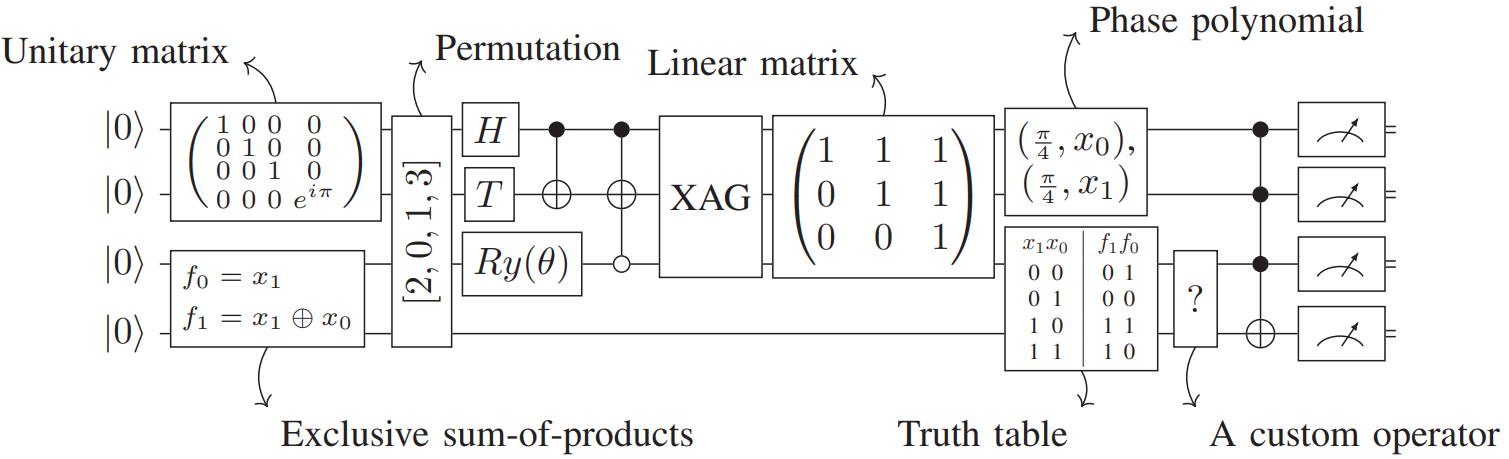
\includegraphics[width=0.9\textwidth]{flex.png}
    \caption{tweedledum's IR flexibility} 
    \label{fig-flex}
  \end{figure}
\end{frame}
\begin{frame}{synthesis}
  \begin{itemize}
    \item 
  \end{itemize}  
\end{frame}
\begin{frame}{synthesis}
  \begin{figure}[htbq]
    \centering
    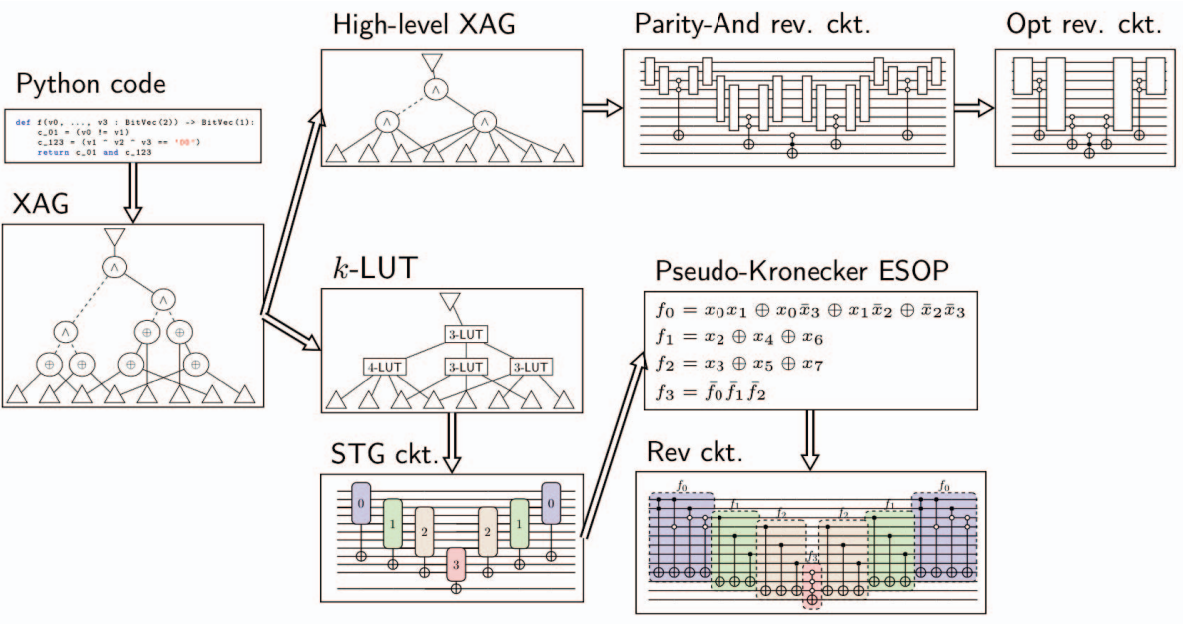
\includegraphics[width=0.7\textwidth]{boolean.png}
    \caption{overview of possible Boolean function synthesis flows} 
    \label{fig-boolean}
  \end{figure}
\end{frame}
\begin{frame}{compilation passes}
  \begin{itemize}
    \item 
  \end{itemize}
\end{frame}
\section*{}
\begin{frame}[noframenumbering,allowframebreaks,t]
	\frametitle{references}
	\printbibliography
\end{frame}
\begin{frame}
\centering
\Huge{END\\Thank you}
\end{frame}
\end{document}